\documentclass[]{standalone}

\usepackage{tikz}
\usepackage{arev}
\usepackage{arevmath}
\usepackage{arevtext}

\begin{document}
  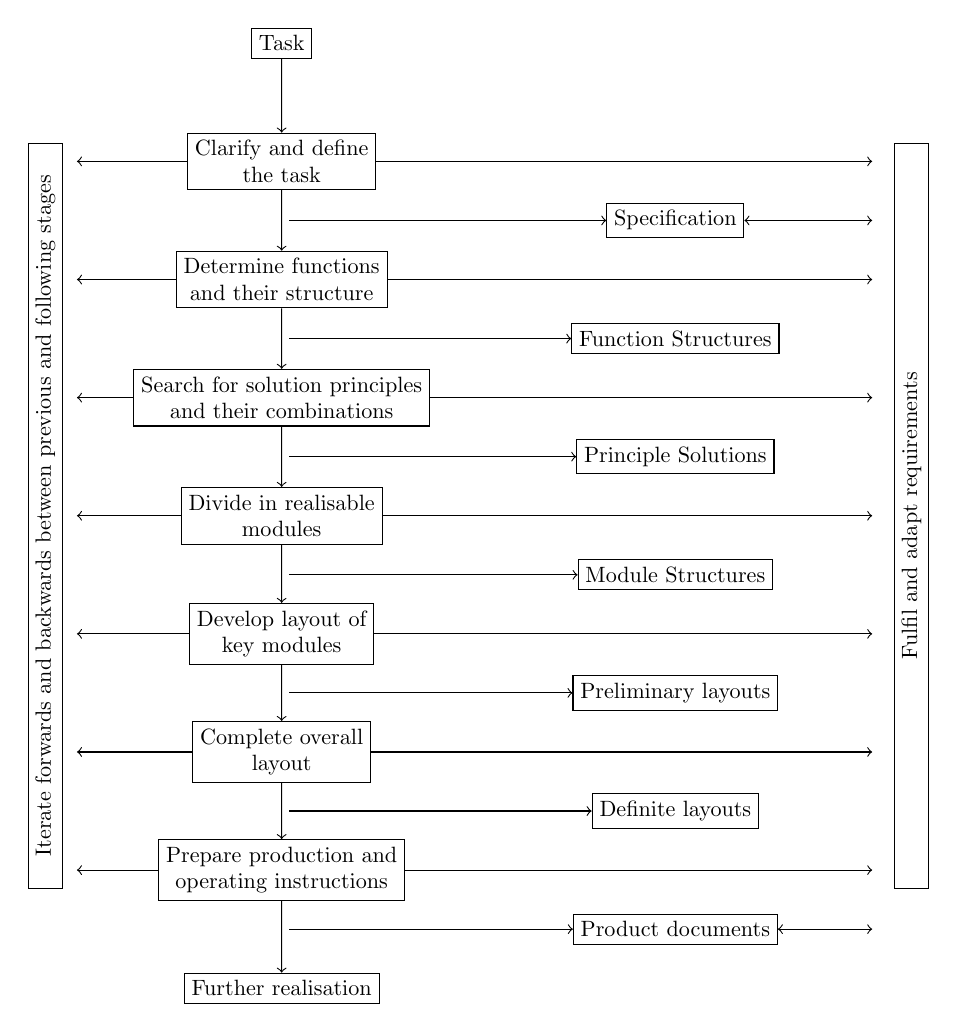
\begin{tikzpicture}[scale=1.0, every node/.style={scale=0.8}]
    \node[align=center, draw] (A) at (0,0) {Task};
    \node[align=center, draw] (B) at (0,-1.5) {Clarify and define\\ the task};
    \draw[->] (A) -- (B);
    \node[align=center, draw] (C) at (0,-3) {Determine functions\\ and their structure};
    \draw[->] (B) -- (C);
    \node[align=center, draw] (D) at (0,-4.5) {Search for solution principles\\ and their combinations};
    \draw[->] (C) -- (D);
    \node[align=center, draw] (E) at (0,-6) {Divide in realisable\\ modules};
    \draw[->] (D) -- (E);
    \node[align=center, draw] (F) at (0,-7.5) {Develop layout of\\ key modules};]
    \draw[->] (E) -- (F);
    \node[align=center, draw] (G) at (0,-9) {Complete overall\\ layout};
    \draw[->] (F) -- (G);
    \node[align=center, draw] (H) at (0,-10.5) {Prepare production and\\ operating instructions};
    \draw[->] (G) -- (H);
    \node[align=center, draw] (I) at (0,-12) {Further realisation};
    \draw[->] (H) -- (I);

    \node[] (AB) at (0,-2.25) {};
    \node[align=center, draw] (J) at (5,-2.25) {Specification};
    \draw[->] (AB) -- (J);

    \node[] (BC) at (0,-3.75) {};
    \node[align=center, draw] (K) at (5,-3.75) {Function Structures};
    \draw[->] (BC) -- (K);

    \node[] (CD) at (0,-5.25) {};
    \node[align=center, draw] (L) at (5,-5.25) {Principle Solutions};
    \draw[->] (CD) -- (L);

    \node[] (DE) at (0,-6.75) {};
    \node[align=center, draw] (M) at (5,-6.75) {Module Structures};
    \draw[->] (DE) -- (M);

    \node[] (EF) at (0,-8.25) {};
    \node[align=center, draw] (N) at (5,-8.25) {Preliminary layouts};
    \draw[->] (EF) -- (N);

    \node[] (FG) at (0,-9.75) {};
    \node[align=center, draw] (O) at (5,-9.75) {Definite layouts};
    \draw[->] (FG) -- (O);

    \node[] (GH) at (0,-11.25) {};
    \node[align=center, draw] (P) at (5,-11.25) {Product documents};
    \draw[->] (GH) -- (P);

    \node[align=center, draw, rotate=90, text width=330] (Q) at (-3,-6) {Iterate forwards and backwards between previous and following stages};
    \draw[->] (B) -- (-2.6,-1.5);
    \draw[->] (C) -- (-2.6,-3);
    \draw[->] (D) -- (-2.6,-4.5);
    \draw[->] (E) -- (-2.6,-6);
    \draw[->] (F) -- (-2.6,-7.5);
    \draw[->] (G) -- (-2.6,-9);
    \draw[->] (H) -- (-2.6,-10.5);

    \node[align=center, draw, rotate=90, text width=330] (Q) at (8,-6) {Fulfil and adapt requirements};
    \draw[->] (B) -- (7.5,-1.5);
    \draw[->] (C) -- (7.5,-3);
    \draw[->] (D) -- (7.5,-4.5);
    \draw[->] (E) -- (7.5,-6);
    \draw[->] (F) -- (7.5,-7.5);
    \draw[->] (G) -- (7.5,-9);
    \draw[->] (H) -- (7.5,-10.5);

    \draw[<->] (P) -- (7.5,-11.25);
    \draw[<->] (J) -- (7.5,-2.25);

  \end{tikzpicture}
\end{document}